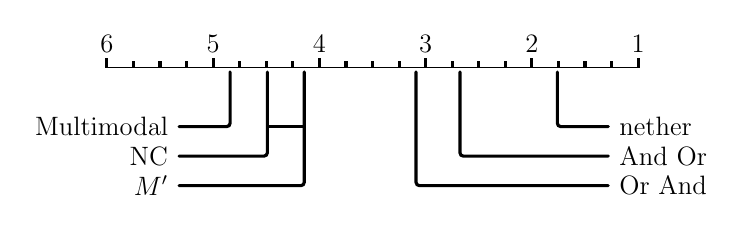
\begin{tikzpicture}[
  treatment line/.style={rounded corners=1.5pt, line cap=round, shorten >=1pt, line width=.5mm},
  treatment label/.style={font=\large},
  group line/.style={ultra thick},
  scale={0.8},
]

\begin{axis}[
  clip={false},
  axis x line={center},
  axis y line={none},
  axis line style={-},
  xmin={1},
  ymax={0},
  scale only axis={true},
  width={\axisdefaultwidth},
  ticklabel style={anchor=south, yshift=1.3*\pgfkeysvalueof{/pgfplots/major tick length}, font=\large},
  every tick/.style={draw=black, line width=.5mm},
  major tick style={yshift=.5*\pgfkeysvalueof{/pgfplots/major tick length}},
  minor tick style={yshift=.5*\pgfkeysvalueof{/pgfplots/minor tick length}},
  title style={yshift=\baselineskip},
  xmax={6},
  ymin={-4.5},
  height={5\baselineskip},
  xtick={1,2,3,4,5,6},
  minor x tick num={3},
  x dir={reverse},
]

\draw[treatment line] ([yshift=-2pt] axis cs:1.7604166666666667, 0) |- (axis cs:1.2604166666666667, -2.0)
  node[treatment label, anchor=west] {nether};
\draw[treatment line] ([yshift=-2pt] axis cs:2.6770833333333335, 0) |- (axis cs:1.2604166666666667, -3.0)
  node[treatment label, anchor=west] {And Or};
\draw[treatment line] ([yshift=-2pt] axis cs:3.0902777777777777, 0) |- (axis cs:1.2604166666666667, -4.0)
  node[treatment label, anchor=west] {Or And};
\draw[treatment line] ([yshift=-2pt] axis cs:4.142361111111111, 0) |- (axis cs:5.340277777777778, -4.0)
  node[treatment label, anchor=east] {$M'$};
\draw[treatment line] ([yshift=-2pt] axis cs:4.489583333333333, 0) |- (axis cs:5.340277777777778, -3.0)
  node[treatment label, anchor=east] {NC};
\draw[treatment line] ([yshift=-2pt] axis cs:4.840277777777778, 0) |- (axis cs:5.340277777777778, -2.0)
  node[treatment label, anchor=east] {Multimodal};
\draw[group line] (axis cs:4.142361111111111, -2.0) -- (axis cs:4.489583333333333, -2.0);

\end{axis}
\end{tikzpicture}